
% This LaTeX was auto-generated from an M-file by MATLAB.
% To make changes, update the M-file and republish this document.

\documentclass{article}
\usepackage{graphicx}
\usepackage{color}

\sloppy
\definecolor{lightgray}{gray}{0.5}
\setlength{\parindent}{0pt}

\begin{document}

    
    
\subsection*{Contents}

\begin{itemize}
\setlength{\itemsep}{-1ex}
   \item Initial configuration
   \item Plots to help see relation between glucose and insulin and ins:glu ratio
   \item Generate stats and graphs between lean and obese controls
   \item Final formatting and save to pdf file
\end{itemize}
\begin{verbatim}
%TREATMENTEFFECTS Test whether the population distributions are normal then
%calculates differential stats for comparing across tretament groups and
%produces the figures to show differences in distributions.
\end{verbatim}


\subsection*{Initial configuration}

\begin{verbatim}
close all
clear all
path(path,'./support_scripts/')

%set filename and path to the file on your computer
[metaboliteFileName, otuFileName] = fileNameCheck('results2.txt', 'otu_table3.txt');

%separate variables
[mconditionStr, metaboliteName, metabolite] = separateMetaboliteVars(metaboliteFileName);

%add insulin:gluose ratio
for i=1:59
    metabolite(27,i)=metabolite(18,i)/metabolite(1,i);
end

%correct metabolite labels
metaboliteName{1} = 'glucose';
metaboliteName{18} = 'insulin';
metaboliteName{27}='insulin:glucose';

%compute averages and errors
[norm, maverages, mstderrors, mcategory] = metaboliteBasicstats(metabolite,mconditionStr);

%compute t-test p value between lean and high dose gram negative
% this could aslo be done with log values, however, the result should
% essentially be the same if not less significant
[hvalue, pvalue]=ttest2(mcategory{1,2}{27,2},mcategory{4,2}{27,2});
\end{verbatim}


\subsection*{Plots to help see relation between glucose and insulin and ins:glu ratio}

\begin{verbatim}
weight_loss_figure;
% figure
% groupcategory=[ones(10,1) ; ones(10,1)+1 ; ones(9,1)+2 ; ones(10,1)+3 ; ones(10,1)+4 ; ones(10,1)+5];
% xax=metabolite(1,:)';
% yax=metabolite(18,:)';
% gscatter(xax,yax,groupcategory,'bgrcmk','*',15);
% figure
% xax=1:59
% plotyy(xax,metabolite(1,:),xax,metabolite(18,:));
% figure
% plotyy(xax,metabolite(18,:),xax,metabolite(27,:));

%n x p
% set up p variable for delta weight and total GLP
weight = [weightchange(:,1); weightchange(:,2);weightchange(1:9,3);weightchange(:,6);weightchange(:,8);weightchange(:,9)];
aglp=metabolite(25,:);
tglp=metabolite(26,:);
X=[ones(length(weight),1) weight metabolite(1:26,:)'];
y=metabolite(27,:)';

j=1;
metaboliteName1{1}='intersect';
for i=1:length(metaboliteName)
        metaboliteName1{i+1}=metaboliteName{i};
end
for i=1:length(y)
    if (isnan(y(i)))
    else
        y1(j)=y(i);
        X1(j,:)=X(i,:);
        j=j+1;
    end
end

% model insulin resistance
mdl2=stepwiselm(X1,y1,'PEnter',0.06,'ResponseVar','insulin resistence','PredictorVars',metaboliteName1);
%[b,se,pval,stats]=stepwiselm(X1,y1, 'display', 'on');
\end{verbatim}

        \color{lightgray} \begin{verbatim}
ans =

  Columns 1 through 7

   26.8200   40.6700   40.3200   39.9900   40.5300   40.9700   40.8900

  Columns 8 through 9

   40.1600   40.4800


ans =

  Columns 1 through 7

   28.0400   41.4300   39.6333   39.3800   40.3222   36.7100   39.0333

  Columns 8 through 9

   38.9600   35.9000


ans =

  Columns 1 through 7

    3.2800   15.5900   15.3000   15.2100   15.4500   15.5400   15.6200

  Columns 8 through 9

   15.2700   15.2600


ans =

  Columns 1 through 7

    3.7400   15.9900   14.1444   13.9400   14.6778   11.6400   13.9667

  Columns 8 through 9

   14.3800   11.2100


mmn =

    -1


mmn =

    -1

BW p value:L

p =

    0.0012

baseline corrected BW p value:L

p =

    0.9405

fat p value:L

p =

   1.4563e-04

baseline corrected fat p value:L

p =

    0.4344

BW p value:O

p =

    0.1204

baseline corrected BW p value:O

p =

    0.3466

fat p value:O

p =

    0.4193

baseline corrected fat p value:O

p =

    1.0000

BW p value:A_{500}

p =

    0.3122

baseline corrected BW p value:A_{500}

p =

    0.0150

fat p value:A_{500}

p =

    0.0806

baseline corrected fat p value:A_{500}

p =

    0.0226

BW p value:A_{150}

p =

    0.0989

baseline corrected BW p value:A_{150}

p =

   4.0022e-04

fat p value:A_{150}

p =

    0.0011

baseline corrected fat p value:A_{150}

p =

   1.5989e-04

BW p value:A_{50}

p =

    0.9633

baseline corrected BW p value:A_{50}

p =

    0.0361

fat p value:A_{50}

p =

    0.0957

baseline corrected fat p value:A_{50}

p =

    0.0151

BW p value:B_{500}

p =

   1.7575e-08

baseline corrected BW p value:B_{500}

p =

   1.9618e-09

fat p value:B_{500}

p =

   1.2767e-07

baseline corrected fat p value:B_{500}

p =

   5.4573e-08

BW p value:B_{150}

p =

    0.0083

baseline corrected BW p value:B_{150}

p =

   3.6601e-04

fat p value:B_{150}

p =

    0.0023

baseline corrected fat p value:B_{150}

p =

   5.5893e-04

BW p value:B_{50}

p =

    0.1210

baseline corrected BW p value:B_{50}

p =

    0.0076

fat p value:B_{50}

p =

    0.2118

baseline corrected fat p value:B_{50}

p =

    0.0832

BW p value:D_{10%}

p =

   1.5054e-06

baseline corrected BW p value:D_{10%}

p =

   2.0597e-07

fat p value:D_{10%}

p =

   3.6407e-07

baseline corrected fat p value:D_{10%}

p =

   1.6156e-07

unpaired t-test for delta weight against obese control:A_{500}

h =

     0


p =

    0.0726

unpaired t-test for delta weight against obese control:A_{150}

h =

     1


p =

    0.0234

unpaired t-test for delta weight against obese control:A_{50}

h =

     0


p =

    0.2683

unpaired t-test for delta weight against obese control:B_{500}

h =

     1


p =

   8.1375e-09

unpaired t-test for delta weight against obese control:B_{150}

h =

     1


p =

    0.0016

unpaired t-test for delta weight against obese control:B_{50}

h =

     1


p =

    0.0295

unpaired t-test for delta weight against obese control:D_{10%}

h =

     1


p =

   5.9830e-08

1. Adding Amylin, FStat = 406.3868, pValue = 1.807879e-24
2. Adding NEFA   mEq/L, FStat = 160.5211, pValue = 1.914427e-16
3. Adding NEFA   mEq/L:Amylin, FStat = 195.1909, pValue = 8.777328e-18
\end{verbatim} \color{black}
    
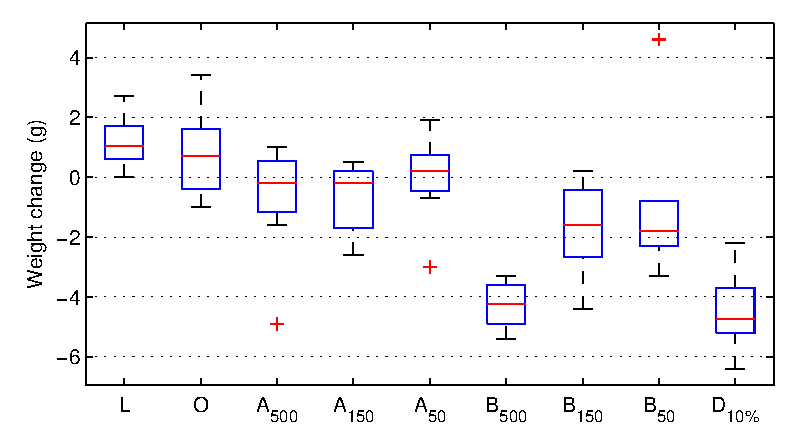
\includegraphics [width=4in]{treatmenteffcts_01.eps}

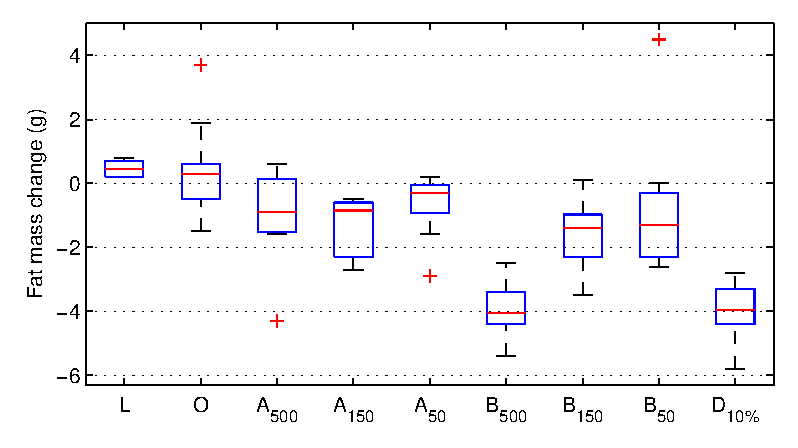
\includegraphics [width=4in]{treatmenteffcts_02.eps}


\subsection*{Generate stats and graphs between lean and obese controls}

\begin{verbatim}
%graphs and stats for glucose (1) insulin (18) active GLP-1 (25) total
%GLP-1 (26) and insulin:glucose ratio (27). Matrix indexes in brackets.
variableIndex = [1 18 25 26 27];
logswitch = [0 0 0 0 0];

%treatment groups: Lean control (1) obese control (2) gram positive
%antibiotic (3) high dose gram negative anitbiotic (4) low dose gram
%negative antibiotic (5) olligofructosccharide supplement (6)
%groups = [1 2 3 4 5 6];
groups = [2 3 4 5 6];

%plot graphs horizontally or vertically
horizontal=0;

%normalisation tests
[h1, hs1] = normalisationTest(variableIndex, mcategory, norm, metaboliteName, logswitch, groups, horizontal);

%box plots and stats
[pvalues, string_answers, h2, hs2] = generateBoxPlotsAndAnovaPValue(variableIndex, mcategory, metaboliteName, logswitch, groups);
\end{verbatim}

        \color{lightgray} \begin{verbatim}
h1 =

     3

    'glucose Lean 0.87055'

    'glucose Vehicle 0.61212'

    'glucose Vancomycin 0.79858'

    'glucose Ceftazadine_low 0.97961'

    'glucose Ceftazadine_high 0.87915'

    'insulin Lean 0.33031'

    'insulin Vehicle 0.90642'

    'insulin Vancomycin 0.61477'

    'insulin Ceftazadine_low 0.9891'

    'insulin Ceftazadine_high 0.88017'

    'active GLP-1 Lean 0.98174'

    'active GLP-1 Vehicle 0.88755'

    'active GLP-1 Vancomycin 0.6058'

    'active GLP-1 Ceftazadine_low 0.57942'

    'active GLP-1 Ceftazadine_high 0.73583'

    'total GLP-1 Lean 0.89778'

    'total GLP-1 Vehicle 0.40209'

    'total GLP-1 Vancomycin 0.95099'

    'total GLP-1 Ceftazadine_low 0.57479'

    'total GLP-1 Ceftazadine_high 0.5291'

    'insulin:glucose Lean 0.28108'

    'insulin:glucose Vehicle 0.90987'

    'insulin:glucose Vancomycin 0.27855'

    'insulin:glucose Ceftazadine_low 0.82367'

    'insulin:glucose Ceftazadine_high 0.99903'


h2 =

     4


hs2 =

   1.0410e+03

    'glucose 0.0019484'


hs2 =

   1.0900e+03

    'insulin 0.038103'


hs2 =

   1.1390e+03

    'active GLP-1 1.0051e-08'


hs2 =

   1.1880e+03

    'total GLP-1 1.1242e-11'


hs2 =

   1.2370e+03

    'insulin:glucose 0.1594'

\end{verbatim} \color{black}
    
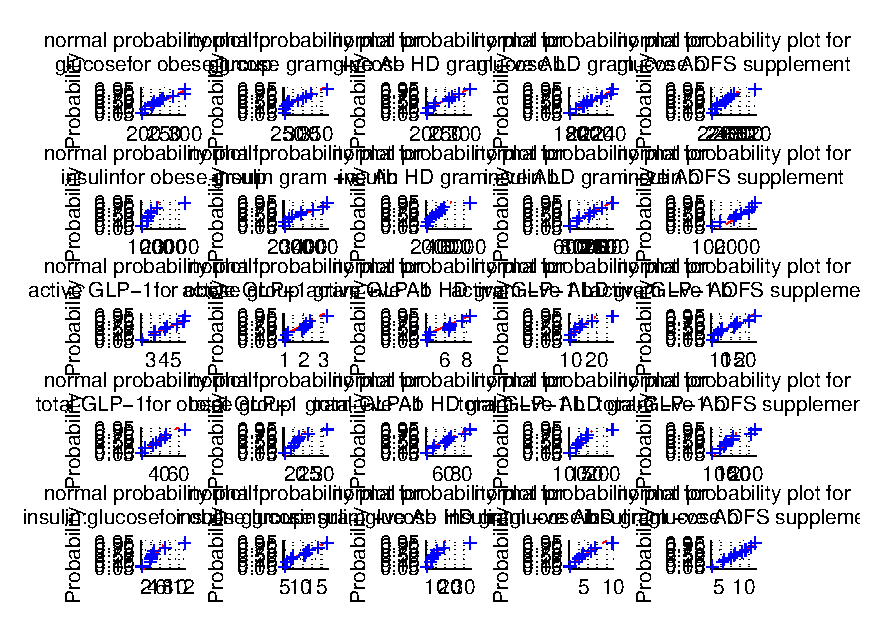
\includegraphics [width=4in]{treatmenteffcts_03.eps}

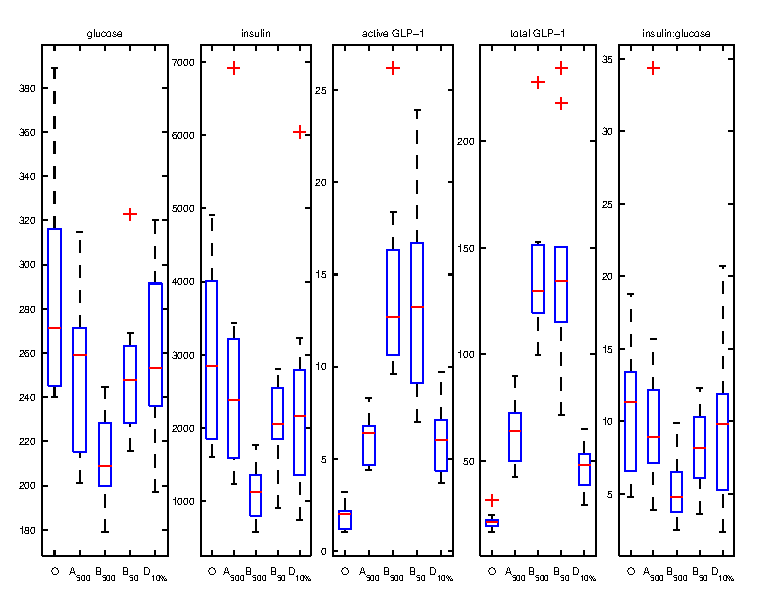
\includegraphics [width=4in]{treatmenteffcts_04.eps}


\subsection*{Final formatting and save to pdf file}

\begin{verbatim}
figure(h1)
% axesHandles = get(gcf,'children');
% set(axesHandles,'fontsize', 5)
% for i=1:length(axesHandles)
%     title = get(axesHandles(i), 'title');
%     set(title, 'fontsize', 7)
%     ylabel(axesHandles(i),'Probability')
% end
%figuresize(15, 10, 'centimeters') %updated script using Matt's magic number!
saveas(gcf, 'pdf_figures/tretamenteffects_diabetic_markers_normalisation_test', 'pdf')

figure(h2)
figuresize(15, 10, 'centimeters')
axesHandles = get(gcf,'children');
%set(h2, 'fontsize', 7)
for i=1:length(axesHandles)
     title = get(axesHandles(i), 'title');
     set(title, 'fontsize', 8)
%      ylabel(axesHandles(i),'Probability')
 end
%set(axesHandles,'fontsize', 10)
saveas(gcf, 'pdf_figures/treatment_effects_diabetic_markers', 'pdf')
\end{verbatim}

        \color{lightgray} \begin{verbatim}
mmn =

    -1

\end{verbatim} \color{black}
    
\includegraphics [width=4in]{treatmenteffcts_05.eps}

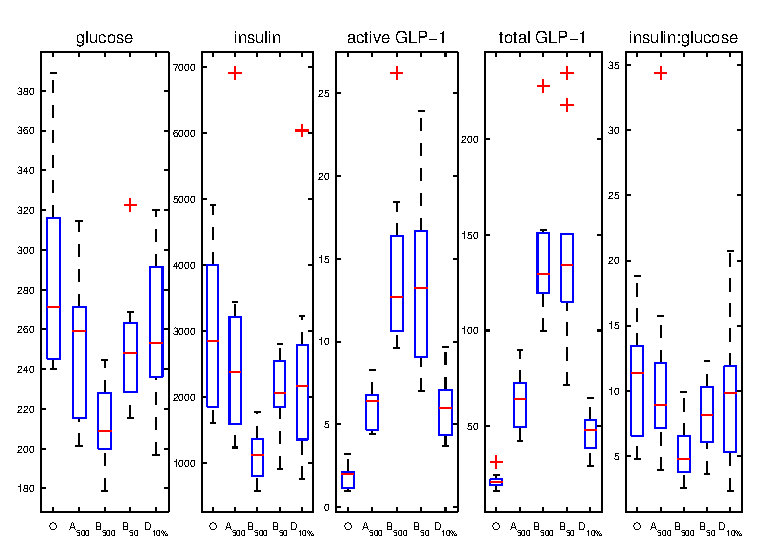
\includegraphics [width=4in]{treatmenteffcts_06.eps}



\end{document}
    
